\documentclass{beamer}

\setbeamertemplate{bibliography item}{\insertbiblabel}
\setlength{\parskip}{\bigskipamount}

\newcommand{\blue}[1]{\textcolor{blue}{#1}}
\newcommand{\red}[1]{\textcolor{red}{#1}}

\title{COMP390: Evolving a Sorting Algorithm with SNGP}
\author{Robin Lockyer}
\institute{University of Liverpool}
\date{03/2019}



\begin{document}
	
	\frame{\titlepage}
	
	\frame{\tableofcontents}
	
	\section{Introduction}
	
		\begin{frame}
		
			\frametitle{Project Description}
			
			Aims:
			
			\begin{itemize}
				
				\item Replicate K. E. Kinnear's work \cite{kinnear_evolving_1993} in evolving a sorting algorithm using Genetic Programming
				
				\pause
				
				\item Re-implement Kinnear's work using Single Node Genetic Programming, a variant of GP invented by Dr David Jackson \cite{jackson_new_2012}
				
				\pause
				
				\item Compare the effectiveness of the two approaches to evolving a sorting algorithm
				 
			\end{itemize}
			
			
		\end{frame}
	
		\begin{frame}
		
			\frametitle{\center{What Was Achieved?}}
			
			Successfully replicated Kinnear's work
			
			\pause
			
			Unable to evolve a sort using SNGP
			
		\end{frame}
	
	\section{Overview of Genetic Programming}
		
		\begin{frame}
		
			\frametitle{What is genetic programming?}
			
			Genetic programming is applying genetic algorithms to programmes in order
			to generate a programme that performs well in a given problem domain.
		
		\end{frame}
	
		\begin{frame}
		
			\frametitle{How Does GP Work? - 1}
			
			Programmes are encoded as a tree of primitive functions and terminals
			
			\begin{center}
				
				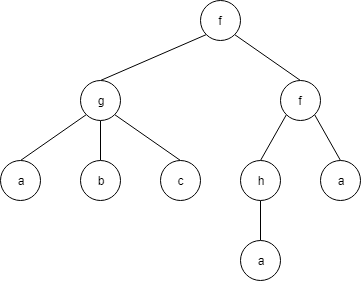
\includegraphics[scale=0.5]{resources/1_gp_example_tree}
				
				This tree encodes the programme f( g( a, b, c ), f( h( a ), a ) ), where f, g, and h are functions and a, b, and c are terminals.
				
			\end{center}
			
			
		
		\end{frame}
	
		\begin{frame}
			
			\frametitle{How does GP Work? - 2}
			
			\begin{center}
				
				An initial population of random programmes is created
				
				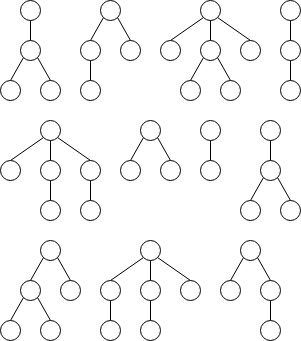
\includegraphics[scale=0.4]{resources/2_gp_example_population}
				
			\end{center}
			
		\end{frame}
	
		\begin{frame}
		
			\frametitle{How Does GP Work? - 2}
			
			\begin{center}
				
				An initial population of random programmes is created
				
				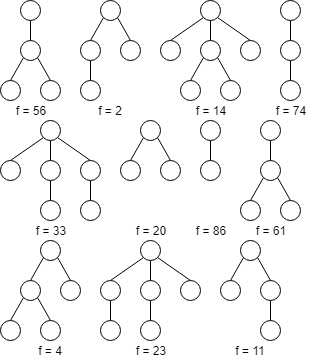
\includegraphics[scale=0.4]{resources/3_gp_example_fitness}
				
				Each member of the population is executed, evaluated, and given a fitness score
				
			\end{center}
			
		\end{frame}
	
		\begin{frame}
		
			\frametitle{How Does GP Work? - 3}
			
			\begin{center}
			
				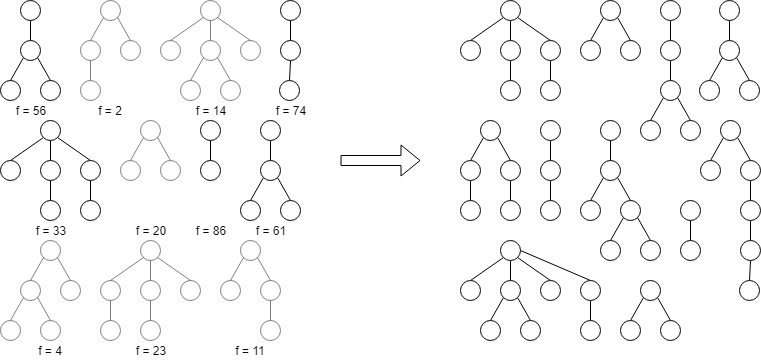
\includegraphics[scale=0.4]{resources/4_gp_example_selection}
				
				A new population is created by selecting some of the most fit members of the initial population and performing genetic operations on them to create new programmes
				
			\end{center}
		
		\end{frame}
	
		\begin{frame}
			
			\frametitle{How Does GP Work? - 4}
			
			There are three main genetic operators:
			
			\medskip
			\pause
			
			\begin{columns}[T]
				
				\begin{column}{0.2\textwidth}
					
					\blue{Reproduction}
					
					\medskip
					
					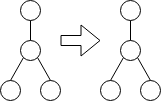
\includegraphics[scale=0.35]{resources/5_reproduction}
					
					\begin{small}
						A programme is copied over to the new population without any changes
					\end{small}
				
				\end{column}
			
				\pause
			
				\begin{column}{0.4\textwidth}
					
					\blue{Crossover}
					
					\medskip
					
					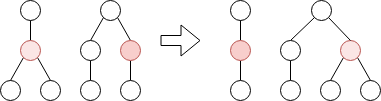
\includegraphics[scale=0.35]{resources/6_crossover}
					\begin{small}
						A random node is selected in each of the chosen programmes. The subtrees rooted at the selected nodes are swapped.
					\end{small}
			
				\end{column}
			
				\pause
			
				\begin{column}{0.3\textwidth}
					
					\blue{Mutation}
					
					\medskip
					
					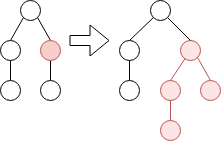
\includegraphics[scale=0.35]{resources/7_mutation}
					
					\begin{small}
						A random node is selected in the chosen programme. A new, random subtree is generated to replace the subtree rooted at the selected node.
					\end{small}
				\end{column}
				
			\end{columns}
			
		\end{frame}
	
		\begin{frame}
		
			\frametitle{How Does GP Work - 5}
			
			This process is repeated until a programme with high enough fitness is generated
		
		\end{frame}
	
	
	\section{Overview of Single Node Genetic Programming}

		\begin{frame}
			
			\large{\blue{What is SNGP?}}
			
			\medskip
			
			\pause
			
			\begin{itemize}
				\item SNGP is a variation of GP that organises the whole population into a single interlinked graph
				
				\pause
				
				\item The subtree rooted at each node in the graph is considered to be an individual programme
				
				\pause
				
				\item The graph is structured in such a way that a form of dynamic programming can be used to increase the efficiency of evaluating the population
			\end{itemize}
			
		\end{frame}
	
		\begin{frame}
		
			\frametitle{SNGP Population - 1}
			
			\center{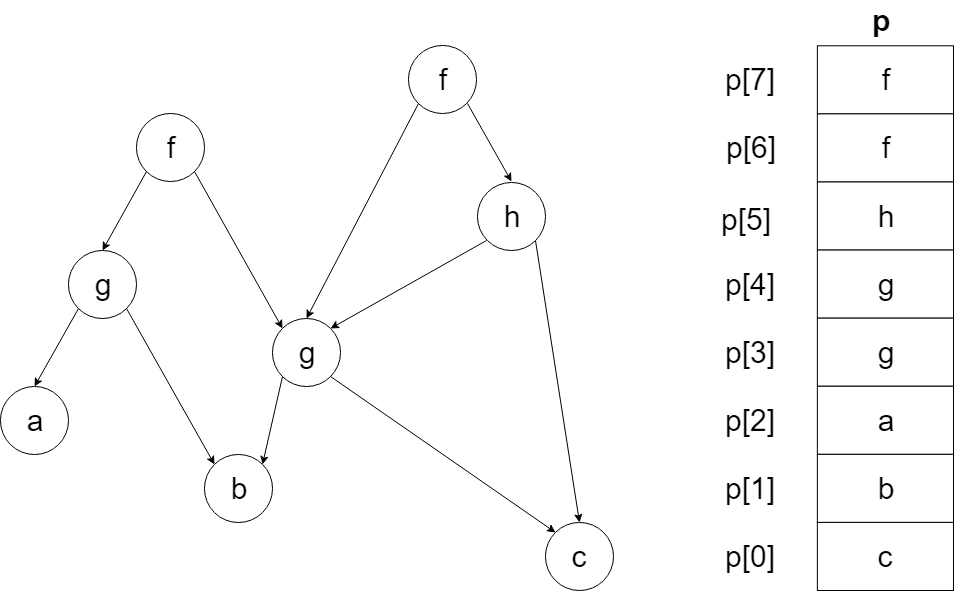
\includegraphics[scale=0.7]{resources/8_sngp_graph}}
					
			\begin{itemize}
				\pause
				\item Graph nodes are stored in an array
				\pause
				\item Terminals are stored in lowest elements
				\pause
				\item Remaining elements store random function
				\pause
				\item Each functions operands are chosen from elements with a smaller index
			\end{itemize}
				
		
		\end{frame}
	
		\begin{frame}
			\frametitle{SNGP Population - 2}
			
			\begin{columns}
				
				\begin{column}{0.4\textwidth}
					
					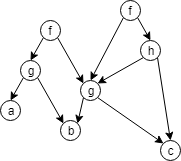
\includegraphics[scale=0.7]{resources/9_sngp_graph_no_array}
					
				\end{column}
			
				\begin{column}{0.6\textwidth}
					
					This graph contains the following programmes:
					
					\begin{itemize}
						\item a
						\item b
						\item c
						\item g( b, c )
						\item g( a, b )
						\item h( g( b, c ), c )
						\item f( g( a, b ), g( b, c ) )
						\item f( g( b, c ), h( g( b, c ), c ) )
					\end{itemize}
					
				\end{column}
				
			\end{columns}
			
		\end{frame}
	
		\begin{frame}
			\frametitle{SNGP Operators}
			
			SNGP has only one genetic operator:
			
			\begin{center}
				
				\blue{Successor Mutate}
				
				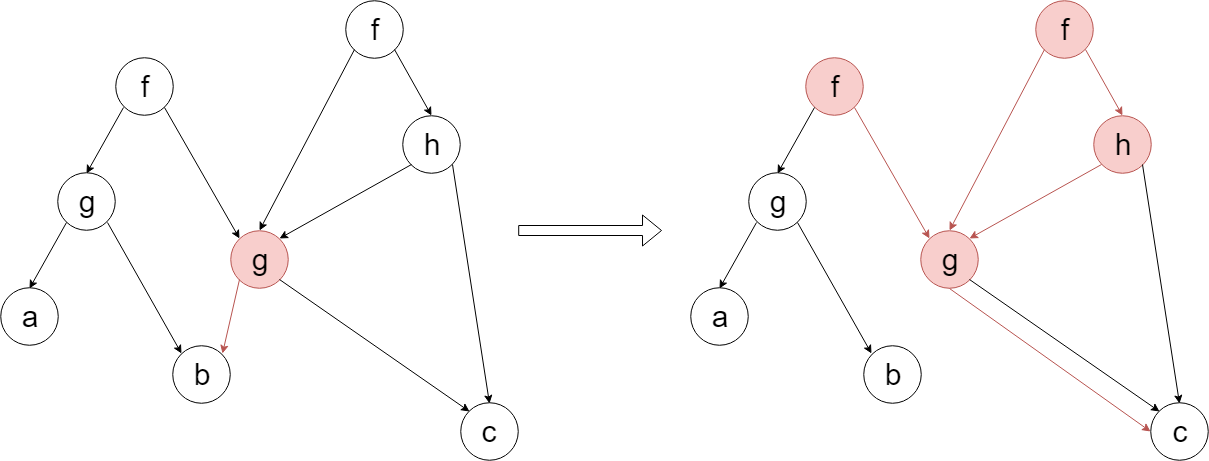
\includegraphics[scale=0.5]{resources/10_successor_mutate}
				
				A random node is chosen and one of its operands is randomly changed. This causes the programmes represented by both the chosen node and all of its predecessors to be altered.
				
			\end{center}
			
		\end{frame}
	
	\section{Reproducing Kinnear's Results}
	
	\section{Attempting SNGP}
	
	\section{Conclusion}
	
	\section{Bibliography}
	
		\begin{frame}
			\frametitle{Bibliography}
			\bibliographystyle{acm}
			\bibliography{library}
		\end{frame}
		
\end{document}